%================================================================
\chapter{Inference on Hodgkin-Huxley}\label{chap:res_hh}
%================================================================  

In this chapter, we present the results from simulation-based inference on the Hodgkin-Huxley (HH) model's conductance parameters $\gbarK$ and $\gbarNa$. 

%\url{https://github.com/mackelab/sbi/blob/main/examples/00_HH_simulator.ipynb}

%Chapter Inference on the HH model 

%- observed data (clean)
%- priors
%- prior predictive sum stats 
%- rej-abc analysis 
%- rej-abc (original) posteriors 
%- reg adj posteriors
%- ppc 

%- observed data noisy 
%- rej-abc (original) posteriors 
%- reg adj posteriors
%- ppc 

%- sbi

%reproducing AP
%numerical solutions similar
%capture

%================================================================
\section{Observation and Feature Extraction}
%================================================================

Let us assume we current-clamped a neuron and recorded the voltage trace in \autoref{fig:hh_obs_data}. This voltage trace was not actually measured experimentally but synthetically generated by simulating the HH model through the HH simulator in \cw{NeuroModels}. The model was simulated for $T=120\ms$ with step size $\Delta t =10 \ms$ and stimulus $I = 10 \, \mathrm{\mu A/cm}^2$ turned on at $10 \ms$ and off at $110 \ms$. The conductance parameters were set as $\gbarK=36 \gunit$ and $\gbarNa=120 \gunit$. The rest of the HH model's parametrization is given in \autoref{tab:hh_model_parameters}. The idealized voltage trace recording, free of any noise, will be used as the observed data in our first analyses. Hopefully, we can then more easily assess strengths and weaknesses of the algorithms themselves, and not have the results overshadowed by noisy data. Furthermore, the present trace allows us to verify whether the computational implementations are accurate. The ground truth parameters will therefore be the particular values of $\gbarK$ and $\gbarNa$ used in the simulation.  

By visual inspection of the trace in \autoref{fig:hh_obs_data}, the expected shape of an action potential (AP) is reproduced by the numerical solution, which indicates that the implementation of the simulator is accurate. Moreover, since the voltage trace does not display any unexpected abrupt behavior, the time resolution of $\Delta t=0.025 \ms$ seems to be sufficient. 

\begin{figure}[!htb]
    \centering
    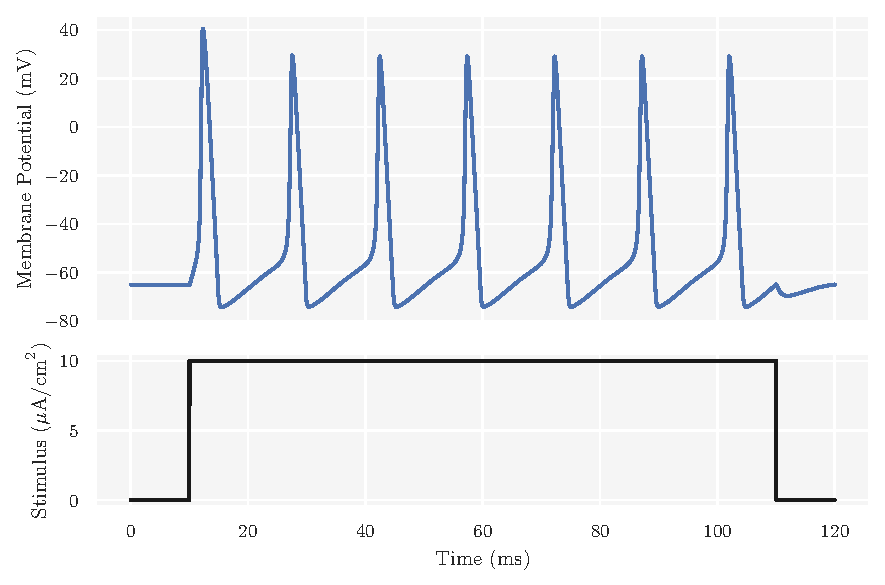
\includegraphics[scale=0.9]{hh_obs_data}
    \caption{Observed voltage trace of a current clamped neuron synthetically generated by the HH simulator simulated for $T = 120 \ms$ with time resolution $\Delta t=0.025 \ms$. The stimulus is a step current $I = 10 \, \mathrm{\mu A/cm}^2$ with onset and offset at $10 \ms$ and $110 \ms$, respectively. Here, the conductance parameters $\gbarK = 36 \gunit$ and $\gbarNa = 120 \gunit$. The present voltage trace being the observation, these conductance parameters are thus the ground truths for the subsequent analyses.}
    \label{fig:hh_obs_data}
\end{figure} 

From the voltage trace, we extract spike statistics by the computational algorithms outlined in \cref{sec:software}. \autoref{fig:hh_stat_extraction} shows the locations in the voltage trace that form the basis of the spike statistic calculations. In fact, the annotations on the voltage trace are set automatically according to the positions found by the extraction algorithms. By the definitions of the different summary statistics provided in \cref{sec:spike_statistics}, we see that the extraction locations are placed correctly on the voltage trace. Consequently, the extraction algorithms seem to function as intended. 

\begin{figure}[!htb]
    \centering
    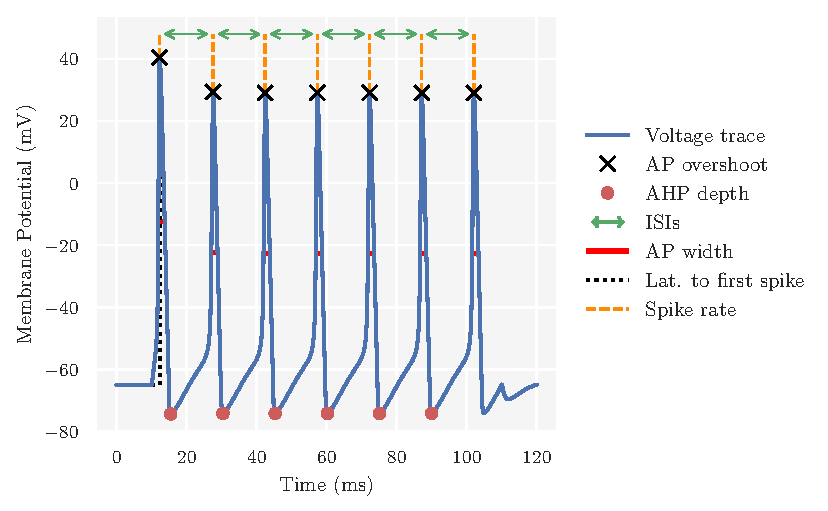
\includegraphics[scale=0.9]{hh_stat_extraction}
    \caption{Locations found by the feature extraction algorithms for spike statistic calculations on the observed voltage trace. The locations are annotated by different markers, with labels stated in the legend, which indicate the particular summary statistic calculation they are affiliated with.}
    \label{fig:hh_stat_extraction}
\end{figure} 

\autoref{tab:hh_obs_sumstats} summarizes the calculated summary statistics from the observed voltage trace; (i) \textit{spike rate}, calculated as the number of spikes divided by the duration of the stimulus; (ii) \textit{average AP overshoot}, calculated by averaging the absolute peak voltage of all APs; (iii) \textit{average AP width}, calculated by averaging the width of every AP at the midpoint between its onset and its peak; (iv) \textit{average AHP depth}, calculated by averaging all minima voltage throughs between two consecutive APs; (v) \textit{latency to first spike}, calculated as the time between stimulus onset and first AP peak; (vi) \textit{accommodation index}, which measures the local variance in ISIs and is calculated by \cref{eq:accomm_index}. Comparing the values of the tabulated summary statistics with the information in \autoref{fig:hh_stat_extraction}, we find agreement. There are 7 spikes over the course of the stimulus duration of $100 \ms$, so the spike rate must be $0.07 \, \mathrm{mHz}$. Furthermore, the value of the average AP overshoot and width, as well as the average AHP depth, seem reasonable when compared with the voltage values at the extracted locations. A latency to first spike of about $2 \ms$ also matches what is seen in the voltage trace. There is practically no difference in length between two consecutive ISIs in the voltage trace, and the accommodation index should therefore reflect, as it does, the lack of variability. All in all, this indicates that also the summary statistic calculations are implemented correctly. 

\begin{table}[!htb]
  \caption{Observed voltage trace reduced to a set of summary statistics. See text for details on the statistics.  }
  %\footnotesize%
  \begin{center}
    \rowcolors{2}{gray!15}{white}
    \begin{tabular}{cc}
      \toprule
      \textbf{Summary statistic} & \textbf{Observed value} \\
      \midrule
      %Number of spikes &  7 \\
      Spike rate &  0.0700 mHz \\
      Average AP overshoot & 30.7316 mV  \\
      Average AP width &  2.0501 mV \\
      Average AHP depth & -74.2234 mV \\
      Latency to first spike & 2.3000 ms \\
      Accommodation index &  $2 \cdot 10^{-17}$ \\
      \bottomrule
    \end{tabular}
  \end{center}
  \label{tab:hh_obs_sumstats}
\end{table}

%================================================================
\subsection{Correlation Analysis \& Importance Weights}
%================================================================

Next, we carry out the correlation analysis outlined in \cref{sec:corr_analysis}. The objective of the analysis is to characterize the effects of parameter variability on the output of the model in terms of the summary statistics. The analysis is done by sampling from the prior predictive distribution, and the priors for $\gbarK$ and $\gbarNa$ are shown in \autoref{fig:hh_priors}. 
\begin{figure}[!htb]
    \centering
    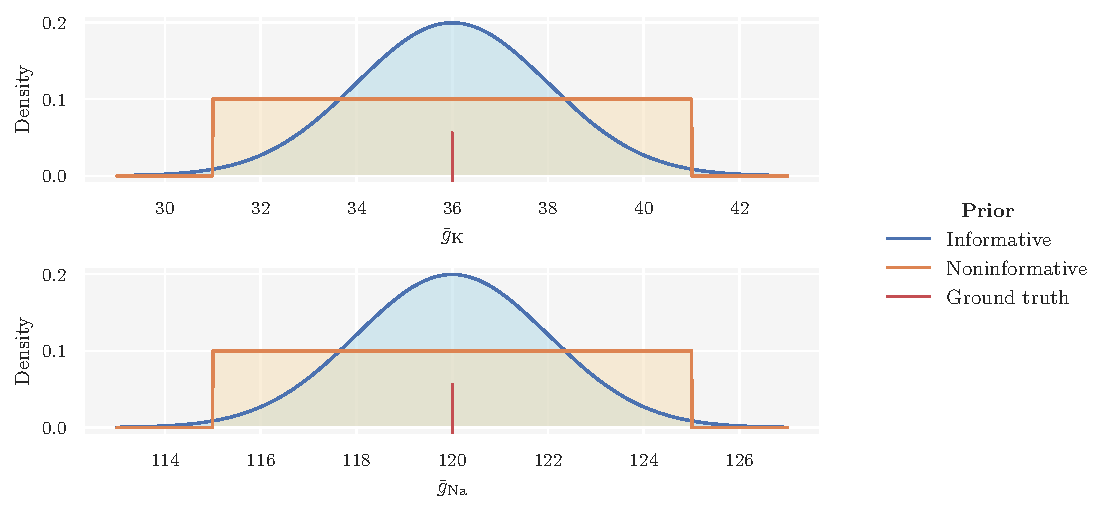
\includegraphics[scale=0.8]{hh_priors}
    \caption{Priors over $\gbarK$ (top) and $\gbarNa$ (bottom). We use both an informative (blue) and noninformative (orange) centered about the ground truth parameter value (red line) for each parameter.}
    \label{fig:hh_priors}
\end{figure}
For each parameter, we use a noninformative prior (orange density) with about $\pm 10\%$ range around the ground truth parameter and a slightly more informative prior (blue density). While technically the informative priors could be classified as weakly-informative (as per the definition given in \cref{sec:coin_flipping}), we will refer to them as informative. 

For each category of priors, we sampled 2000 parameter pairs, fed them to the HH simulator model and calculated the summary statistics from the simulated data for each pair. The spike statistics are only well-defined in the presence of spikes, and accommodation index and average AHP depth need at least two and three spikes, respectively, to be defined. As such, we need to remove samples if they contain ill-defined statistics.

%================================================================
\subsubsection*{With Informative Priors}
%================================================================

Of the 2000 summary statistics samples simulated under the informative priors, 1881 were well-defined. Scatter plots for a subset of these are shown in \autoref{fig:hh_priorpred_sstats_normal}, where the summary statistics are shown as functions of the pairs of parameter values. Thus, the scatter plots enable us to see the variability the different summary statistics exhibit relative to change in model parameter values. Each point indicates the relative magnitude of the statistic by its size and color, with a reference table stated in the legend along with the name of the particular statistic.
\begin{figure}[H]
    \centering
    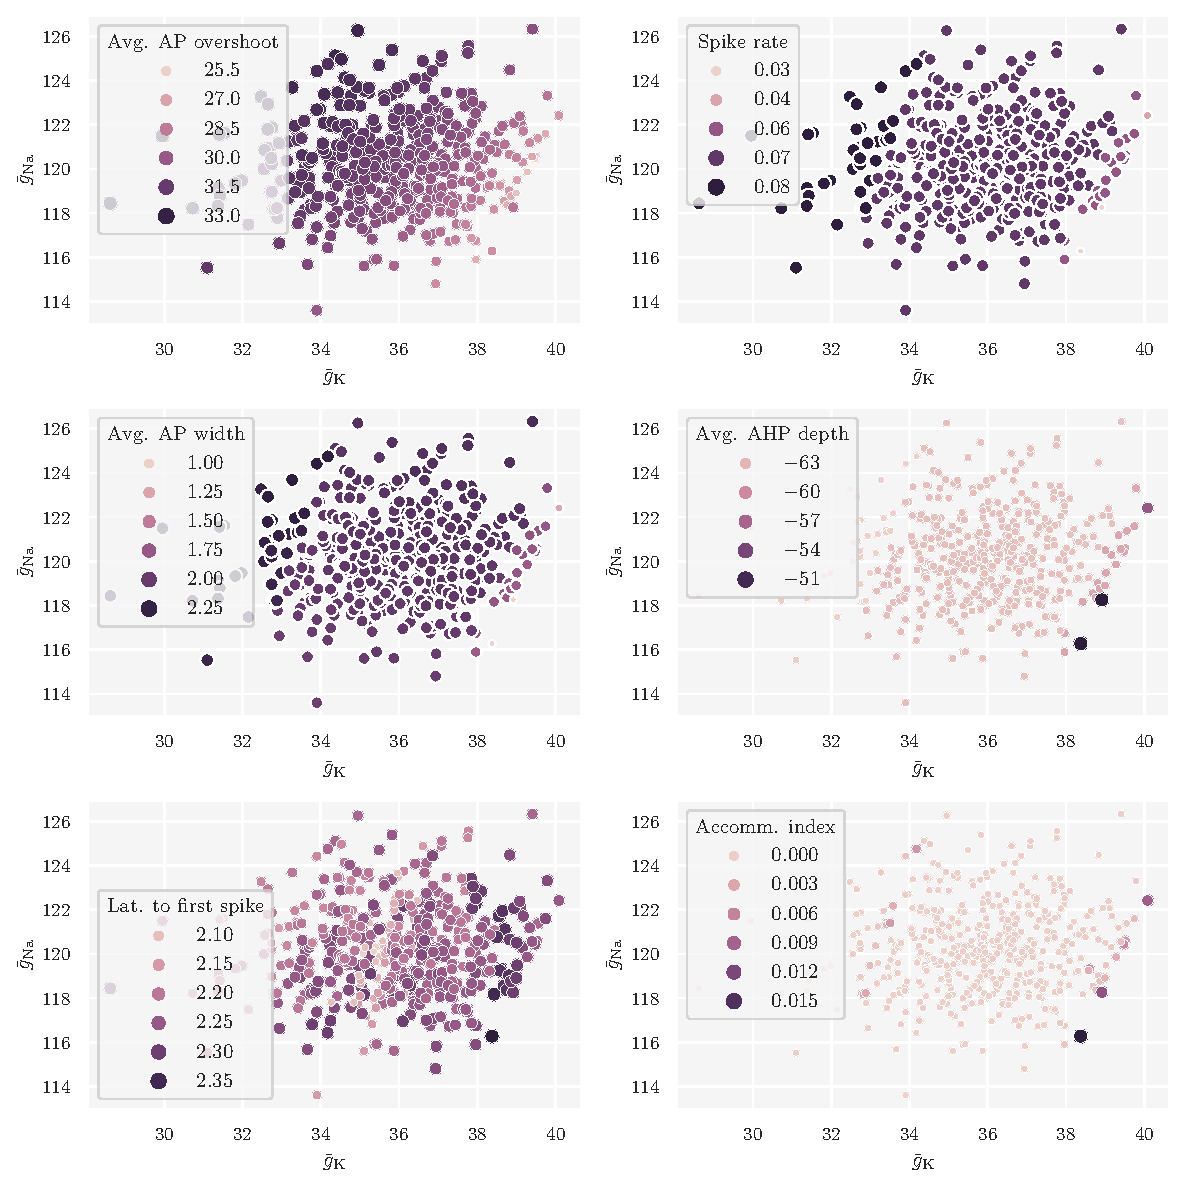
\includegraphics[scale=0.7]{hh_priorpred_sstats_normal}
    \caption{Scatter plots of summary statistics simulated with different pairs of model parameter values. The summary statistics were simulated under the joint informative prior predictive distribution. Of 2000 generated samples, 1881 were well-defined. Here, a subset of 470 samples are shown. Each summary statistic is assigned to its own panel, with the particular statistic stated in the legend. Each point represents the value of a summary statistic for a pair of parameter values, $\qty(\gbarK, \gbarNa)$. The color of a point indicates the relative magnitude of the statistic, for which bright colors represent small and dark colors large values, also indicated in each subplot legend. The scatter plots thus indicate the variability of summary statistics relative to movement of the pairs of model parameter values.
    }
    \label{fig:hh_priorpred_sstats_normal}
\end{figure} 
In addition to displaying the variability, the scatter plots also indicate if there is a systematic relationship between a parameter and summary statistic. By fixing the value of one of the parameters and following its line-of-sight, we can assess whether the other parameter systematically increments or decrements a summary statistic. Average AP overshoot exhibits a steady variability and seems to follow an approximately linear trend. This also applies to the average AP width, though to a lesser extent. The approximate linear relationship is most apparent for $\gbarK$ in both cases. In terms of the underlying biophysical mechanisms, we would expect average AP overshoot to be most sensitive to $\gbarNa$ and average AP width to $\gbarK$. The role of the \Na channel in AP generation is well-established, and AP overshoot is tied to the fast \Na channel dynamics. Likewise, given the role of the \K channel in repolarizing the neuron after an AP, the average AP width is tied to the duration of the recovery period. While these expectations are not clearly present in the scatter plots, we should keep in mind that we only explore a fairly limited region of the parameter space. We should therefore be cautious in our interpretation of how well the scatter plots indicate sensitivity. Accommodation index has almost no variation, which might be unsurprising since it measures the local variance in ISIs. The constant current protocol does not facilitate much variation in spike trains. Thus, for the observed voltage trace at hand, accommodation index is not an informative summary statistic. However, it could be useful in characterizing spike trains generated under more complex current protocols. Average AHP depth also exhibits little variation, whereas latency to first spike an ample amount. Though, for latency to first spike there is no apparent systematic relationship, as it increments and decrements right and left. This might not be optimal for constraining the model parameters. Finally, the spike rate, though it does not vary much, seem to have a more systematic and stable relationship with the model parameters, predominantly $\gbarK$. It behaves more like a step function, where it retains a particular value for a prolonged range of $\gbarK$ values. In conclusion, how well this set of summary statistics will constrain the model parameters needs to be investigated further down the line.  

In order to not rely solely on visual inspection of the sensitivity, \autoref{fig:hh_weights_normal} provides the pairwise Pearson's correlation coefficients of each model parameter and summary statistics, as well as the importance weights derived from the correlation coefficients.
% subfigure
\begin{figure}[!htb]
\centering
\subfloat[]{{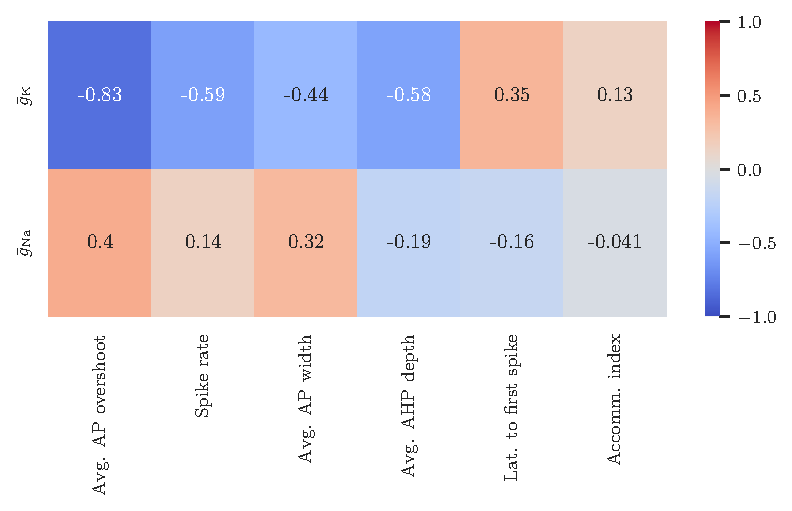
\includegraphics[scale=0.65]{hh_priorpred_corr_normal}}}
\qquad
\subfloat[]{{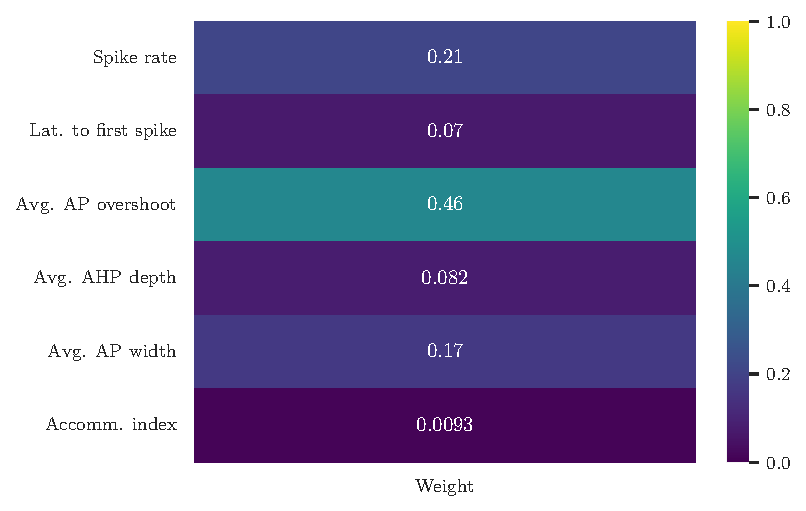
\includegraphics[scale=0.65]{hh_priorpred_weights_normal}}}
\caption{\textbf{(a)} The pairwise Pearson's correlation coefficients for the model parameters and summary statistics. \textbf{(b)} The importance weights calculated from the correlation coefficients, see \cref{sec:corr_analysis} for details. Note that the weights sum to one.
}
\label{fig:hh_weights_normal}
\end{figure}
As was indicated by the scatter plots, $\gbarK$ has a stronger (approximately) linear relationship with the summary statistics than $\gbarNa$. The interpretation of these results are that the summary statistics related to the shape of an AP encode the most information, with average AP overshoot being the most dominant. Moreover, the results indicate that $\gbarK$ will be constrained better than $\gbarNa$ by these summaries when performing regression adjustment. Since the relationship between $\gbarK$ and the summary statistics is much stronger than for $\gbarNa$, the weighting scheme also becomes biased towards $\gbarK$. The weighting is therefore a bit unfair for $\gbarNa$. For instance, even though the spike rate is weakly correlated with $\gbarNa$, it receives a heavy weight because it is strongly correlated with $\gbarK$. The weight of the spike rate even surpasses that of average AP width, which shows a decent amount of correlation with both $\gbarNa$ and $\gbarK$. The pairwise Pearson's correlation coefficients strong assumption about linearity again necessitates the need to be wary of the interpretation of which summary statistics are the most informative. As the weighting scheme prefers $\gbarK$, we should also investigate the effects importance weights have on the inference further down the line.

%================================================================
\subsubsection*{With Noninformative Priors}
%================================================================

The findings with noninformative priors are similar to the ones discussed above. This is perhaps unsurprising, since a prior does not alter the intrinsic relationship between a parameter and summary statistic, just how the samples are distributed in the parameter space. The corresponding figures with samples from the joint noninformative prior distribution can be found in \cref{sec:Appendix A}.


%================================================================
\section{Study of ABC Settings}
%================================================================

We now turn to a study concerning the tuning parameters in the rejection ABC algorithm. As the generation of one posterior amounts to a single stochastic trial, we will generate several posteriors for the same settings in order to assess potential variability in the results. Here, we use the rejection sampler in \cw{pyLFI} to infer the conductance parameters in the HH model. The performance metrics RMSPE and SEM, defined in \cref{sec:performance_metrics}, will be used to assess the accuracy and variability, respectively, of a particular inference setting.

In our first tuning parameter analysis, we study the effect of the tolerance parameter $\epsilon$ in terms of the $p_\epsilon$-quantile of the distances. For each quantile, we generate 10 posterior with 1000 posterior samples in each. As discussed in \cref{sec:software}, this means that the tolerance will be set via a pilot study. For each quantile, the pilot study performs 2000 simulations to estimate both the tolerance and the scale of the summary statistics. In this analysis, the summary statistics are equally weighted. Having obtained a posterior, we perform local linear regression adjustment with the Epanechnikov kernel and log transformation of the parameters to obtain a corresponding adjusted posterior. We do the above using both the informative and noninformative priors. \autoref{fig:RMSPE_vs_quantile} shows the results.
\begin{figure}[!htb]
    \centering
    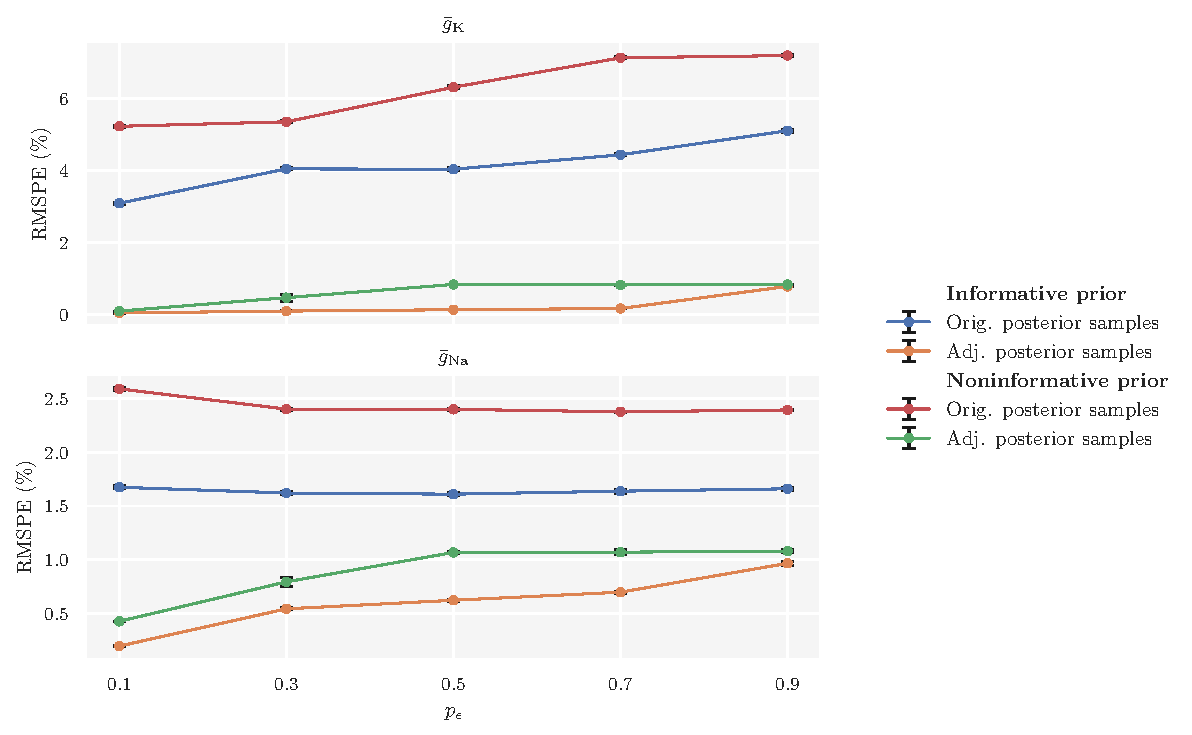
\includegraphics[scale=0.8]{RMSPE_vs_quantile}
    \caption{The RMSPE in posteriors over $\gbarK$ (top) and $\gbarNa$ (bottom) against the $p_\epsilon$-quantile as a measure of tolerance. Each point is the mean RMSPE over 10 posteriors, each consisting of 1000 posterior samples, and the SEM is shown as a vertical bar. The posteriors were generated by the rejection ABC algorithm and then adjusted with local linear regression adjustment. Whether an estimate of error had informative/noninformative priors or is from the original/adjusted posterior is color coded (see legend).}
    \label{fig:RMSPE_vs_quantile}
\end{figure} 
RMSPE measures the percentage difference between the ground truth and a weighted estimate that accounts for the width of the posterior. Increasing $p_\epsilon$-quantiles amount to accepting simulated data that are increasingly further away from the observed data. As such, we expect the error to increase with $p_\epsilon$, due to more distorted approximations. This is also the general trend, though the differences in error between posteriors are generally small. Here, the posterior error estimates of $\gbarK$ and $\gbarNa$ differ. Focusing on the estimates of error in the original posterior samples, i.e., the samples obtained solely with the rejection ABC algorithm, $\gbarK$ has larger errors than $\gbarNa$. The errors of $\gbarNa$ remain almost constant as $p_\epsilon$ increases, and are actually slightly larger for the lowest $p_\epsilon$. The reason for this may be intricate, but most likely it has to do with correlation between the posterior samples of $\gbarNa$ and $\gbarK$ and that the simulated summary statistics accepted under a strict tolerance happen to shift the $\gbarNa$ estimate for the worse (by a little amount) and $\gbarK$ for the better. In terms of variation, the SEM of all the mean RMSPE shows that the inferred posteriors for the same settings are practically indistinguishable. We also see that estimates with informative priors converge better than those with noninformative priors, as expected. The RMSPE of the regression adjusted posterior estimates are significantly more accurate than the original posterior estimates. The improvement is most prominent for $\gbarK$, and aligns with the expectation obtained from the correlation analysis; since $\gbarK$ has a stronger linear relationship with the summary statistics than $\gbarNa$, the local linear regression model will give better adjustment of the $\gbarK$ posterior samples. The difference in error when $p_\epsilon$ increases are tiny for $\gbarK$, which suggests that the regression approach manages to correct the $\gbarK$ samples as if they were sampled from $\pi_\mathrm{ABC} \qty(\gbarK \mid \rho \qty(\ssim, \sobs) \leq \epsilon)$ with $\epsilon=0$. For $\gbarNa$, however, this breaks down and the error increases with $p_\epsilon$, with a particular jump between the 0.1 and 0.5-quantiles. Nevertheless, with regression adjustment, more simulations can be accepted without sacrificing substantial accuracy, especially for the model parameters that are the most constrained by the summary statistics. In addition, the difference in error between using informative and noninformative priors is also reduced when performing regression adjustment. 

Next, we investigate error in the estimates against the number of summary statistics used to constrain the model parameters. We start with only a single statistic, average AP overshoot, and increment by one more according to the following order; spike rate, average AP width, average AHP depth, latency to first spike and accommodation index. Again, we use the quantile-based rejection ABC algorithm with local linear regression adjustment using the Epanechnikov kernel to estimate the posteriors. We use the 0.4-quantile as a compromise between accuracy and run time (see \autoref{fig:runtime}). From the preceding result (\autoref{fig:RMSPE_vs_quantile}) we found that the posteriors generated for the same settings are practically identical. Here, we therefore only generate a single posterior for each number of summary statistics. This is, however, done for both the informative and noninformative priors. In addition, we generate posteriors for both cases of weighting of the summary statistics; either equally or importance weighted (we ensure the importance weights sum to one). The results are shown in \autoref{fig:RMSPE_vs_n_sumstats}.
\begin{figure}[!htb]
    \centering
    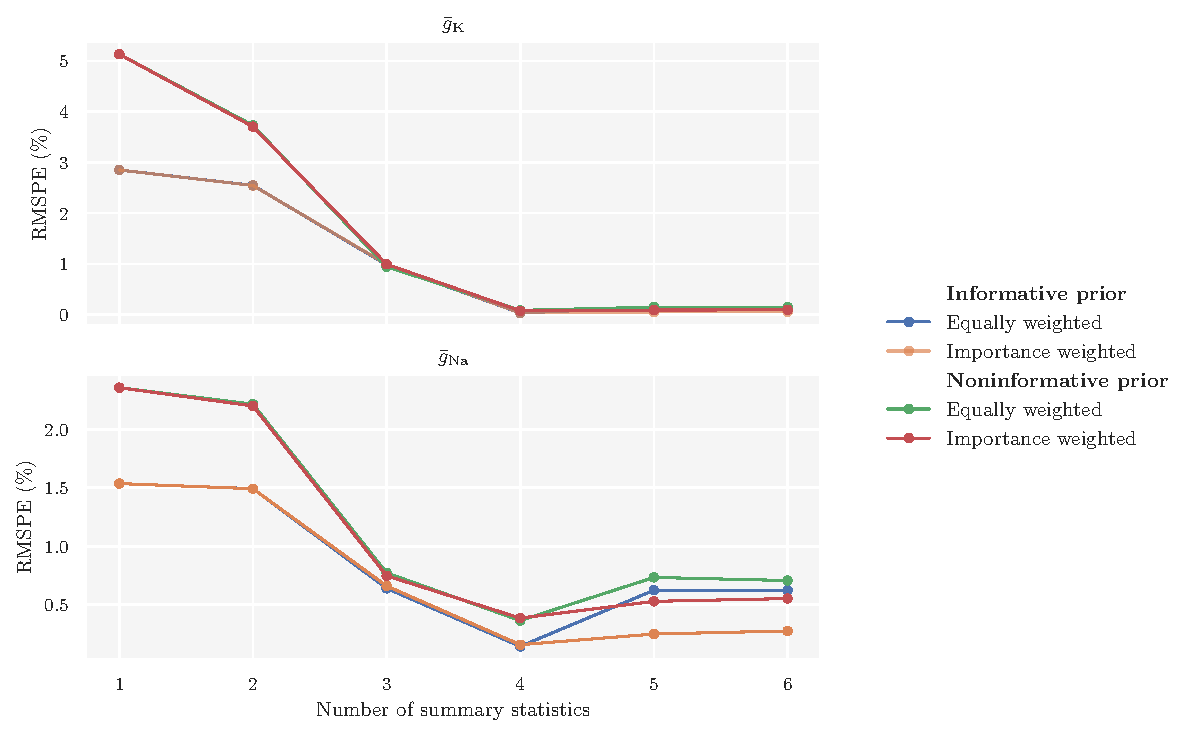
\includegraphics[scale=0.8]{RMSPE_vs_n_sumstats}
    \caption{The RMSPE in posteriors over $\gbarK$ (top) and $\gbarNa$ (bottom) against the number of summary statistics. The first, single statistic is (i) average AP overshoot, and then the number of statistics is incremented by one more according to the following order; (ii) spike rate, (iii) average AP width, (iv) average AHP depth, (v) latency to first spike and (vi) accommodation index. Each point is the RMSPE in a regression adjusted posterior consisting of 1000 posterior samples. Whether an estimate of error had informative/noninformative priors or equally/importance weighted the summary statistics is color coded (see legend).
    }
    \label{fig:RMSPE_vs_n_sumstats}
\end{figure} 
The figure shows that the HH model is more tightly constrained by increasing the number of summary statistics, particularly $\gbarK$ as we have already discussed. Though, if we use summary statistics that do not capture relevant information for the parameters, it might lead to worse inference. The set of summary statistics that gives the most accurate posteriors consists of: (i) average AP overshoot, (ii) spike rate, (iii) average AP width and (iv) average AHP depth. For $\gbarK$, inclusion of the remaining two statistics, (v) latency to first spike and (vi) accommodation index, does not lead to a noticeable difference in accuracy. Neither does using equally or importance weighted summary statistics. For $\gbarNa$, on the other hand, the error becomes moderately worse by including (v) latency to first spike and (vi) accommodation index. Here, using importance weights actually helps to constrain $\gbarNa$ and improves the error in the posterior. 

Informed by the preceding findings, going forward we will use the set of summary statistics labelled (i)-(iv) above and also keep the inclusion of importance weights.


%================================================================
\section{Summarizing Posteriors}
%================================================================

We can assess the identifiability of the HH model's active conductance parameters by examining the locations and widths of the resulting posterior estimates. A wide, flat posterior on a parameter indicates a large number of equally optimal values, which suggests that the parameter may be unidentifiable. As outlined in \cref{sec:performance_metrics}, the goodness of fit of the inferred posteriors will be considered through the MAP estimate, $95\%$ highest density interval (HDI) and, since we have access to the ground truths, RMSPE. We will also use posterior predictive checks to check for auto-consistency. To reiterate the settings of the rejection ABC sampler; we generate the following posteriors using the 0.4-quantile to set the tolerance and the set of importance weighted summary statistics (i) average AP overshoot, (ii) spike rate, (iii) average AP width and (iv) average AHP depth.

\subsection{Posteriors from Informative Priors}

\autoref{fig:hh_posterior_org_normal} shows the original posteriors over $\gbarK$ and $\gbarNa$, with summarizing metrics stated in the legends.
\begin{figure}[H]
    \centering
    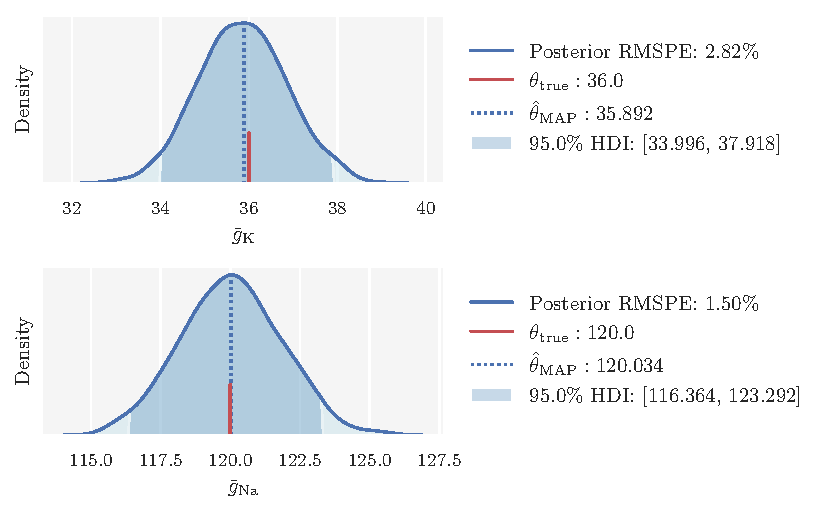
\includegraphics[scale=1]{hh_posterior_org_normal}
    \caption{Original rejection ABC posteriors over the Hodgkin-Huxley model parameters $\gbarK$ (top) and $\gbarNa$ (bottom). Here, the parameter proposals were sampled from the joint informative prior distribution. }
    \label{fig:hh_posterior_org_normal}
\end{figure}
Compared to the (informative) priors over the model parameters (see \autoref{fig:hh_priors}), the updated state of knowledge represented by the posteriors is more constrained. The MAP estimates are centered close on the ground truth parameters, which, by the definition of MAP, means that the ground truth parameters are in regions of high posterior density. Although the posteriors. Compared to the $\gbarNa$ posterior, the RMSPE of the $\gbarK$ posterior is slightly larger, even though the 95\% HDI of $\gbarK$ is narrower than that of $\gbarNa$. This might be a bit surprising, but can be explained by noticing the sharpness of the posterior peaks. The peak of the $\gbarK$ posterior is more flat compared to the peak of the $\gbarNa$ posterior, which is quite sharp about the ground truth, and this is reflected in the RMSPE measure.





ground truth parameter values are in regions of high posterior density 


the analysis revealed that as more features are taken into account, the posterior became narrower and centered more closely on the ground truth parameters



Application of these new techniques also allows us to explore the issue of model identifiability. By examining posterior distributions over model parameters, we can quantify and characterize model uncertainty, which can either inform us as to the ability of our data to constrain the model or the degree of biological variability in the system, as we outline below.

---

Make subfig with corr and joint

Correlation 




---
\autoref{fig:hh_joint}
% subfigure
\begin{figure}[!htb]
\centering
\subfloat[]{{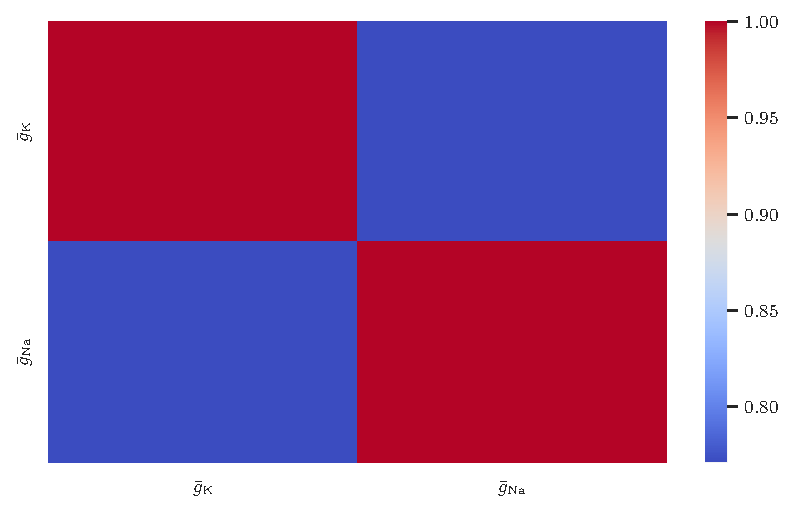
\includegraphics[scale=0.5]{hh_corr_org_normal}}}
\qquad
\subfloat[]{{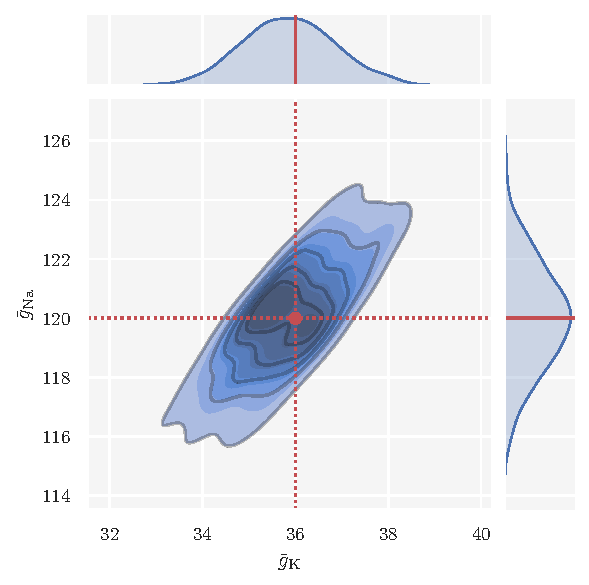
\includegraphics[scale=0.65]{hh_joint_posterior_org_normal}}}
\caption{\textbf{(a)} The pairwise Pearson's correlation coefficients for the posterior samples of $\gbarK$ and $\gbarNa$. \textbf{(b)} The joint posterior distribution of $\gbarK$ and $\gbarNa$. Darker regions correspond to higher density, and the ground truth is indicated by the red marker and axis lines. Since the marginal posteriors over model parameters (shown on the marginal axes) are highly correlated, predictive posterior samples need to be sampled from the joint posterior. 
}
\label{fig:hh_joint}
\end{figure}

---


Posteriors, reg adjusted samples, informative prior

\begin{figure}[H]
    \centering
    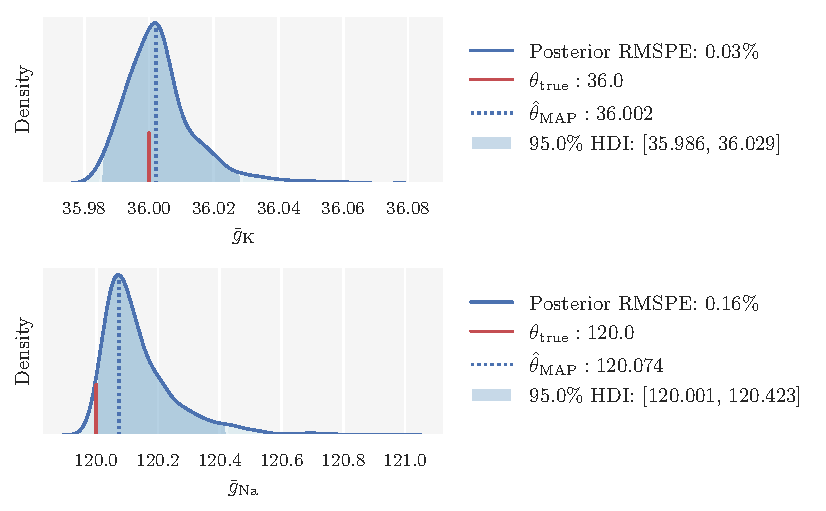
\includegraphics[scale=1.0]{hh_posterior_reg_normal}
    \caption{caption}
    \label{fig:fig1}
\end{figure}

regression adjustment of the posteriors is crucial for obtaining accurate estimates with the rejection ABC sampler. 

PPC reg adjusted posterior predictive 

\begin{figure}[H]
    \centering
    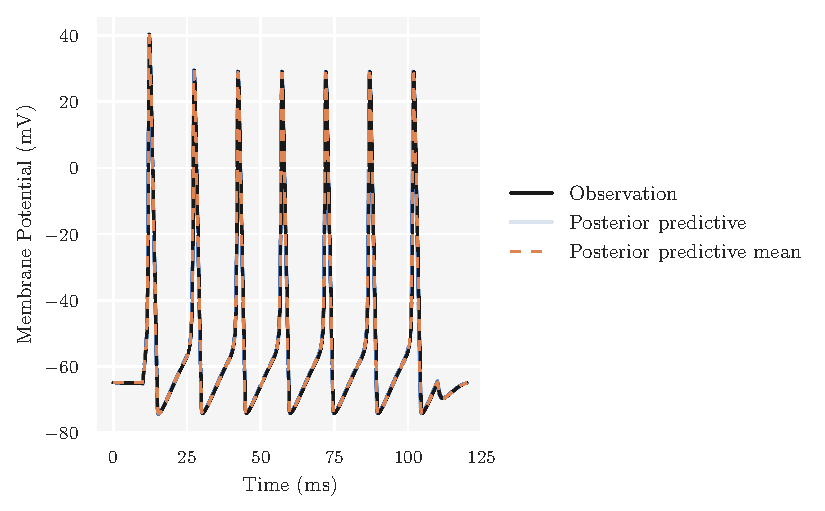
\includegraphics[scale=1.0]{hh_postpred_reg_normal}
    \caption{caption}
    \label{fig:fig1}
\end{figure}


As can be seen, the samples from the inferred posterior lead to simulations that closely resemble the observed data, confirming that Rej-ABC did a good job at capturing the observed data in this simple case.

\subsection{Noninformative priors}

posterior, original, noninfo prior

\begin{figure}[H]
    \centering
    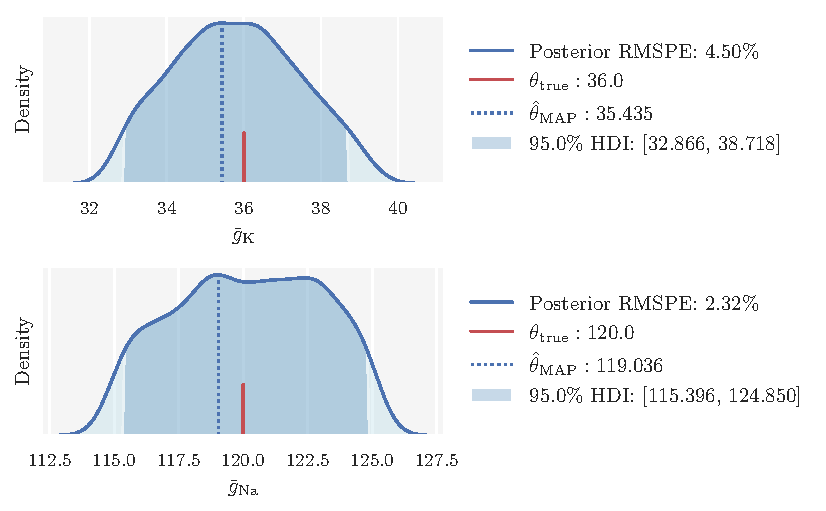
\includegraphics[scale=1.0]{hh_posterior_org_uniform}
    \caption{Original rejection ABC posteriors over the Hodgkin-Huxley model parameters $\gbarK$ (top) and $\gbarNa$ (bottom). Here, the parameter proposals were sampled from a joint noninformative prior distribution.}
    \label{fig:fig1}
\end{figure}

Adjusted posterior, noninformative prior

\begin{figure}[H]
    \centering
    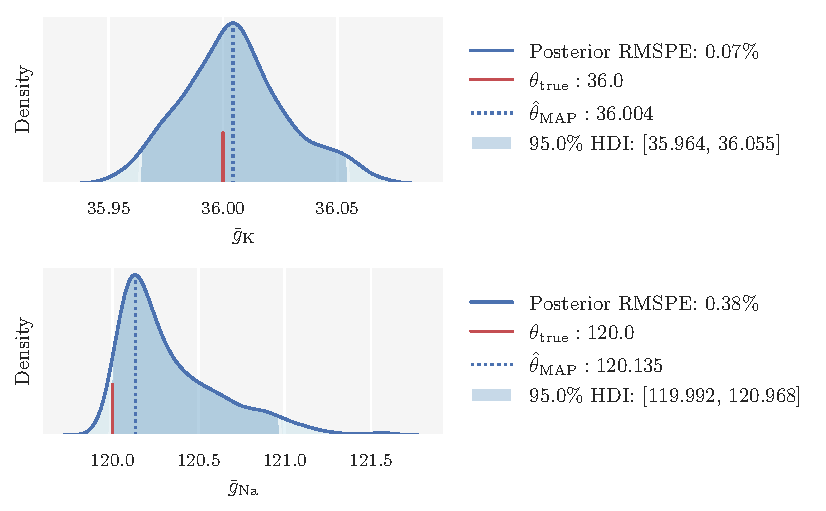
\includegraphics[scale=1.0]{hh_posterior_reg_uniform}
    \caption{caption}
    \label{fig:hh_posterior_reg_uniform}
\end{figure} 

PPC adjusted posterior 

\begin{figure}[H]
    \centering
    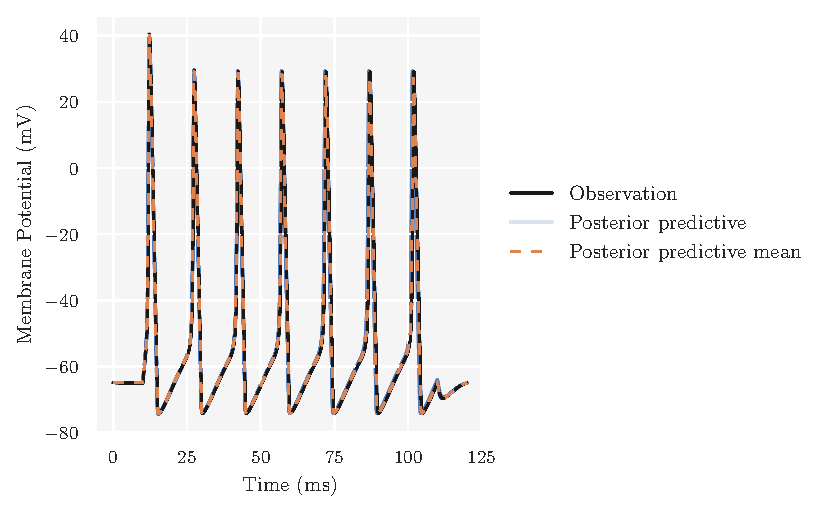
\includegraphics[scale=1.0]{hh_postpred_reg_uniform}
    \caption{Posterior predictive check of the. With predictions sampled from the regression adjusted posterior shown in \autoref{fig:hh_posterior_reg_uniform}}
    \label{fig:fig1}
\end{figure}


%================================================================
\section{HH SBI Results}
%================================================================

same observed data as for clean hh

Posterior:

\begin{figure}[H]
    \centering
    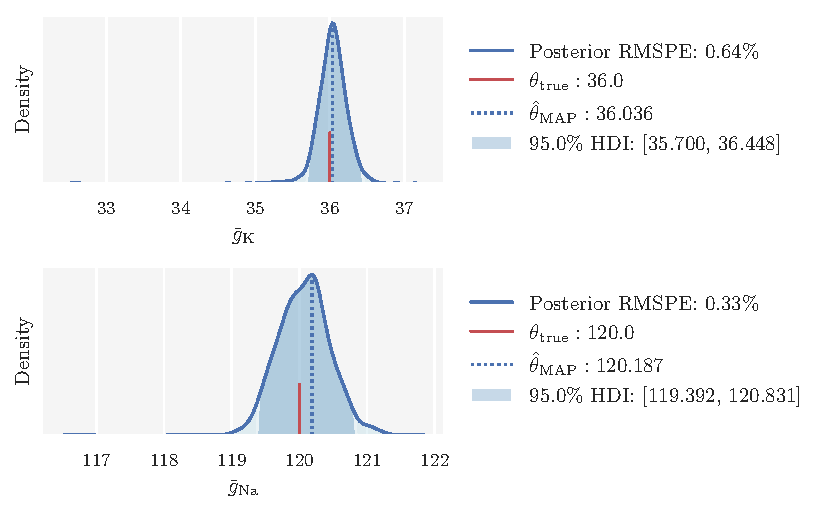
\includegraphics[scale=0.8]{hh_post_sbi}
    \caption{caption}
    \label{fig:fig1}
\end{figure}

%PPC
%\begin{figure}[H]
%    \centering
%    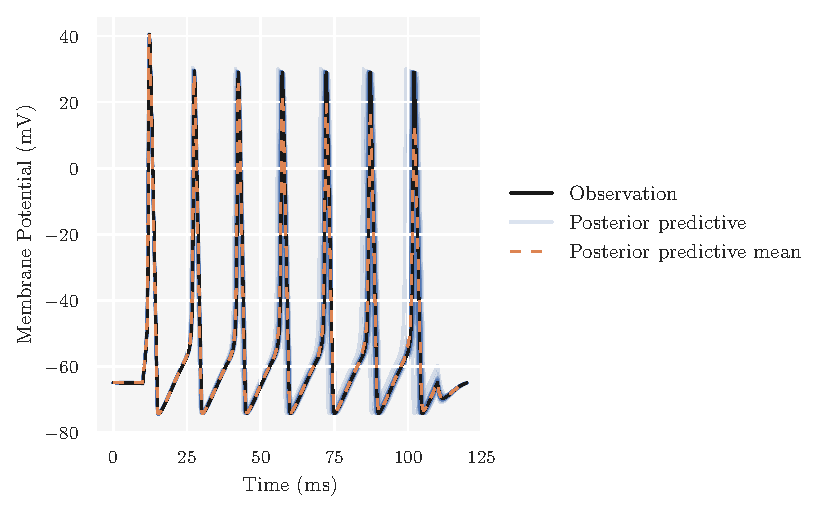
\includegraphics[scale=0.8]{hh_post_pred_sbi}
%    \caption{caption}
%    \label{fig:fig1}
%\end{figure}

%see that the wider posterior has an effect on recreating the observed data, this is not present in rej-abc reg adjust posterior due to it being more narrow


%================================================================
\section{Noisy Observation}
%================================================================

\begin{figure}[H]
    \centering
    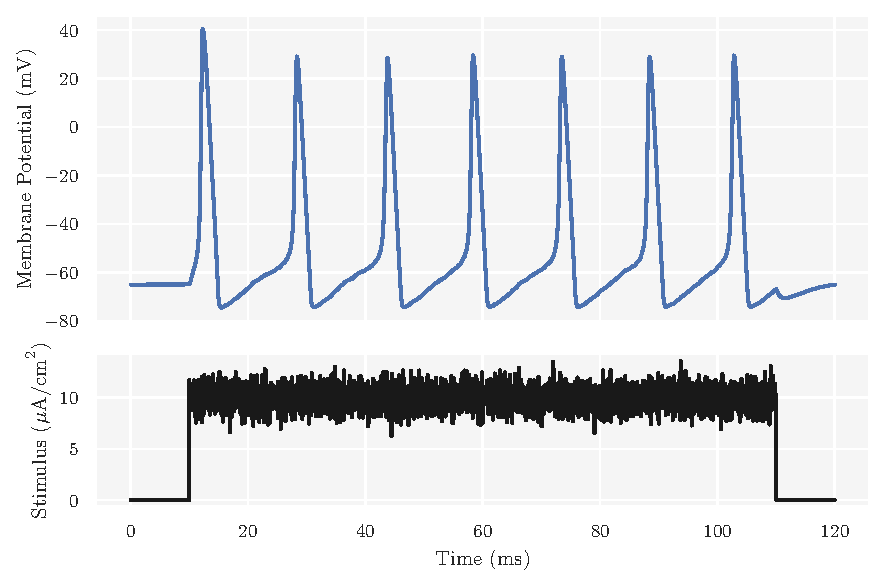
\includegraphics[scale=0.9]{hh_noisy_data}
    \caption{caption}
    \label{fig:fig1}
\end{figure} 


% Alternating row colors
\begin{table}[H]
  \caption{Generic table with alternating rows and different sized rulers. The number of spikes is not used as a summary statistic in and of itself, but is included to show that the statistic extraction indeed finds all spikes.}
  %\footnotesize%
  \begin{center}
    \rowcolors{2}{gray!15}{white}
    \begin{tabular}{cc}
      \toprule
      \textbf{Summary statistic} & \textbf{Observed value} \\
      \midrule
      Number of spikes &  7 \\
      Spike rate &  0.0700 mHz \\
      Average AP overshoot & 30.7223 mV  \\
      Average AP width & 2.0679 mV \\
      Average AHP depth & -74.3394 mV \\
      Latency to first spike & 2.2750 ms \\
      Accommodation index &  -0.0067 \\
      \bottomrule
    \end{tabular}
  \end{center}
  \label{tab:hh_noisy_sumstats}
\end{table}



----

observed data w/o noise 

feature extraction 

plot features 

compute weights (plot correlation matrix) 

plot priors (informative, noninformative)


---

create the observed data

summary statistics of observation 

summary statistics from prior predictive

weights

(observed data with noise; same as above)


original posterior on noisy observed data

\begin{figure}[H]
    \centering
    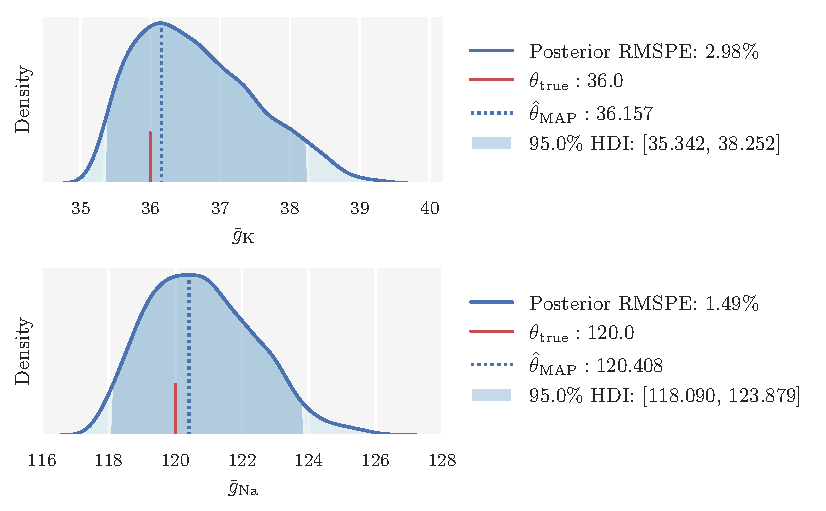
\includegraphics[scale=1.0]{hh_posterior_org_noisy}
    \caption{caption}
    \label{fig:fig1}
\end{figure} 

adjusted posterior on noisy observed data

\begin{figure}[H]
    \centering
    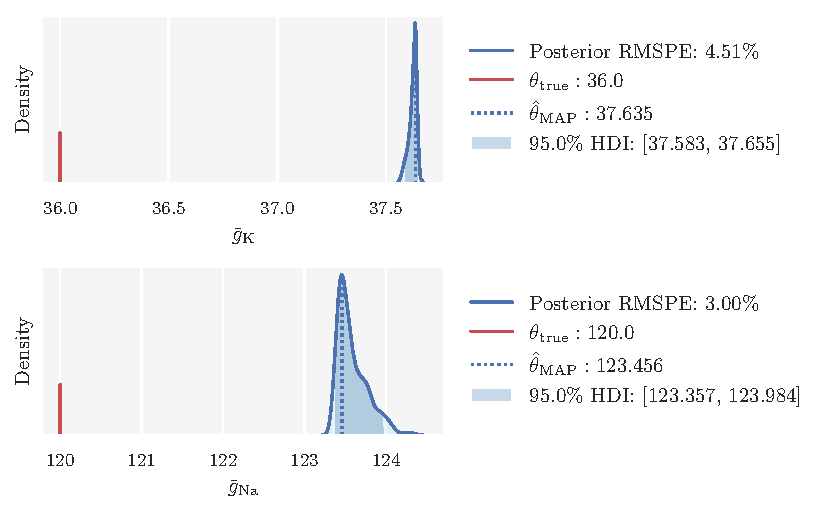
\includegraphics[scale=1.0]{hh_posterior_reg_noisy}
    \caption{caption}
    \label{fig:fig1}
\end{figure} 

ppc with reg adjusted posterior samples (100 posterior samples)


\begin{figure}[H]
    \centering
    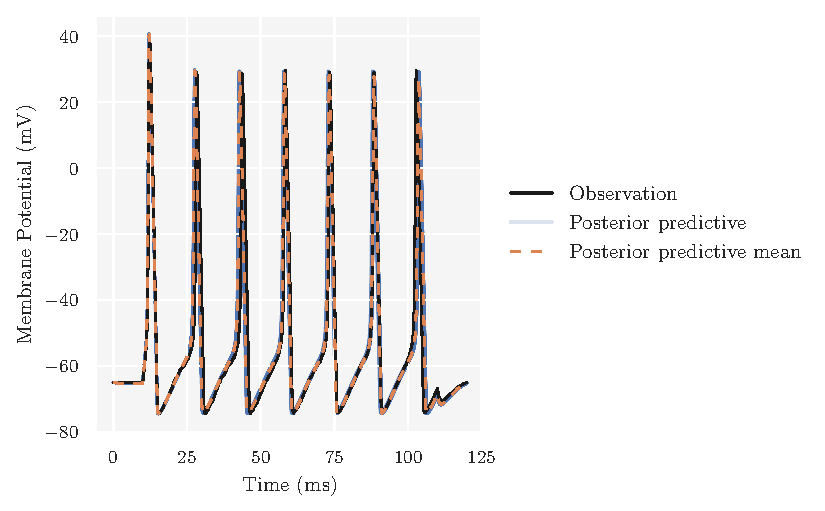
\includegraphics[scale=1.0]{hh_postpred_reg_noisy}
    \caption{caption}
    \label{fig:fig1}
\end{figure}
%================================================================
\chapter{Inference on Brunel}\label{chap:res_brunel}
%================================================================ 

Chapter Inference on the Brunel model
- observed data 
- priors
- prior predictive sum stats 
- rej-abc (original) posteriors 
- reg adj posteriors
- ppc 
- sbi


%%
%%
%%
%%
%%

%================================================================
%\chapter{Analysis of the Hodgkin-Huxley Model}
\chapter{Analysis of the Neuroscientific Models}
%================================================================

lat to first spike, accomm index -> unsurprising, little variation, could perhaps be more useful to characterize spike trains generated under more complex current protocols. 




\textit{accommodation index}, which measures the local variance in ISIs and is calculated by

% chapter: Inference on the Hodgkin-Huxley Model 
% chapter: Inference on the Brunel Model





%================================================================
\section{The Brunel Network Model}
%================================================================

create the observed data

summary statistics of observation 

summary statistics from prior predictive

weights


%================================================================
\chapter{Parameter Identification with REJ-ABC}
%================================================================

%================================================================
\section{Rejection ABC Posteriors on Conductance Parameters}
%================================================================

show how Hodgkin–Huxley model is more tightly constrained by increasing numbers of data features

We also inferred HH parameters for 8 in vitro recordings from the Allen Cell Types database using the same current-clamp stimulation protocol as in our model [60, 70] (Fig. 4F, Supplementary Fig. 8). In each case, simulations based on the SNPE-inferred posterior closely resembled the original data (Fig. 4F). We note that while inferred parameters differed across recordings, some parameters (the spike threshold, the density of sodium channels, the membrane reversal potential and the density of potassium channels) were consistently more strongly constrained than others (the intrinsic neural noise, the adaptation time constant, the density of slow voltage-dependent channels and the leak conductance) (Supplementary Fig. 8). Overall, these results suggest that the electrophysiological responses measured by this current-clamp protocol can be approximated by a single-compartment HH model, and that SNPE can identify the admissible parameters.



%================================================================
%\section{ABC Settings for Identification of Brunel Network Parameters}
%================================================================

%================================================================
%\section{Rejection ABC Posteriors on Synaptic Weight Parameters}
%================================================================

%================================================================
\chapter{Brunel ABC Results}
%================================================================

Brunel 

\section{Observation}

observed spiketrain 

\begin{figure}[H]
    \centering
    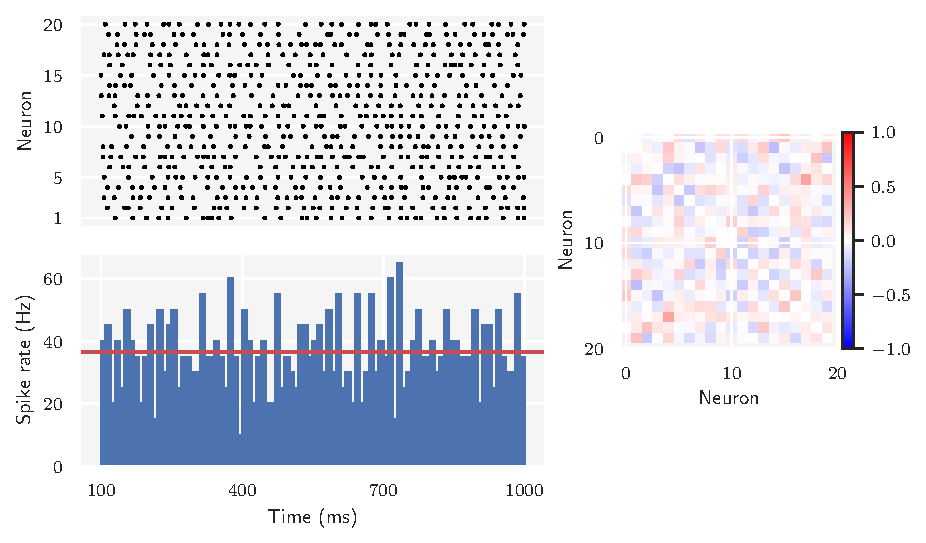
\includegraphics[scale=1.0]{brunel_ai_observation}
    \caption{caption}
    \label{fig:fig1}
\end{figure}

sum stats

% Alternating row colors
\begin{table}[H]
  \caption{AI state observed sum stats}
  %\footnotesize%
  \begin{center}
    \rowcolors{2}{gray!15}{white}
    \begin{tabular}{cc}
      \toprule
      \textbf{Summary statistic} & \textbf{Observed value} \\
      \midrule
      Mean firing rate &  0.0366 kHz \\
      Mean CV &  0.4250  \\
      Fano factor & 0.2341  \\
      \bottomrule
    \end{tabular}
  \end{center}
  \label{tab:hh_noisy_sumstats}
\end{table}

correlation (pearson) coefficient matrix

\begin{figure}[H]
    \centering
    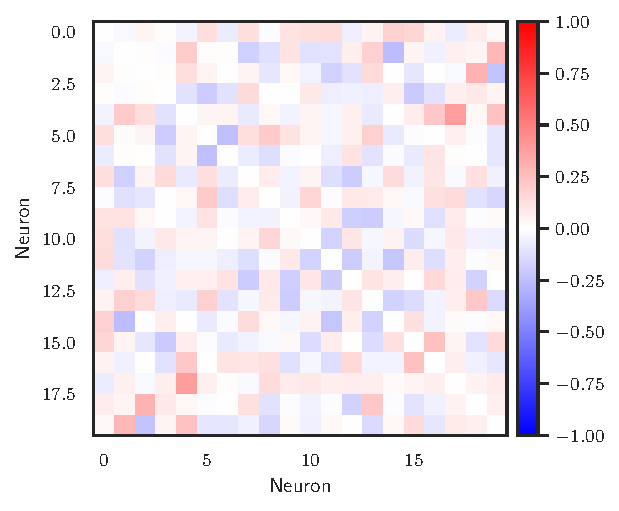
\includegraphics[scale=1.0]{brunel_obs_corr}
    \caption{caption}
    \label{fig:fig1}
\end{figure}

\section{prior pred}

priors

\begin{figure}[H]
    \centering
    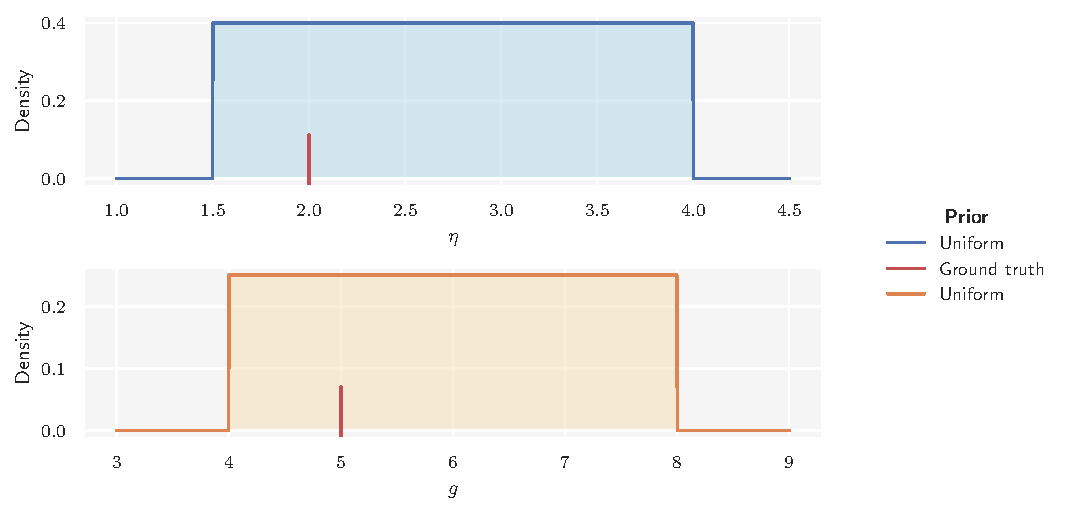
\includegraphics[scale=0.8]{brunel_priors}
    \caption{caption}
    \label{fig:fig1}
\end{figure}

sum stats scatter (500 samples)

\begin{figure}[H]
    \centering
    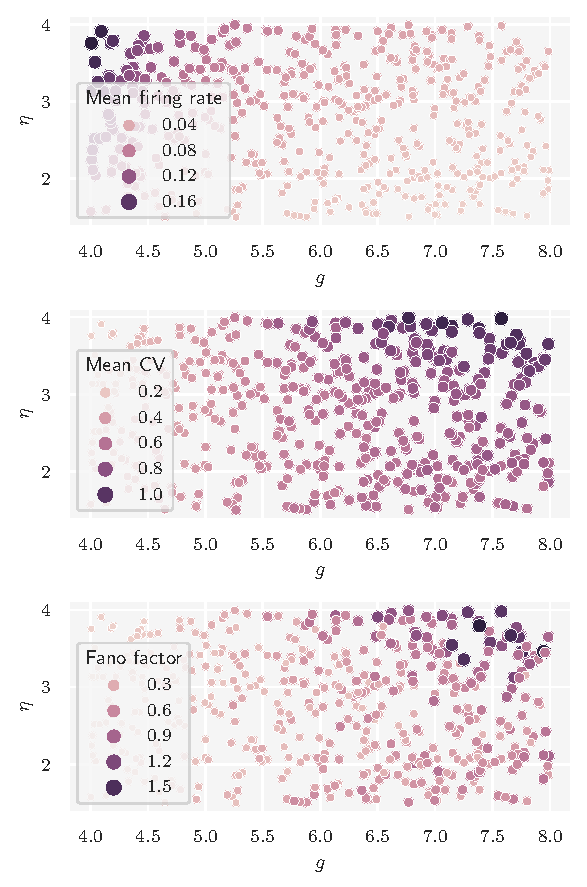
\includegraphics[scale=1.0]{brunel_sum_stats}
    \caption{caption}
    \label{fig:fig1}
\end{figure}


sum stats correlation and weights

% subfigure
\begin{figure}[H]
\centering
\subfloat[]{{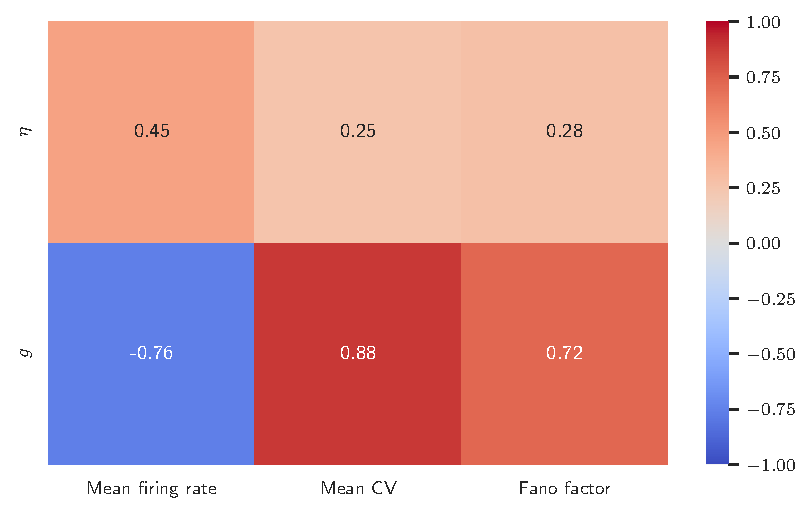
\includegraphics[scale=0.7]{brunel_sum_stats_corr}}}
\qquad
\subfloat[]{{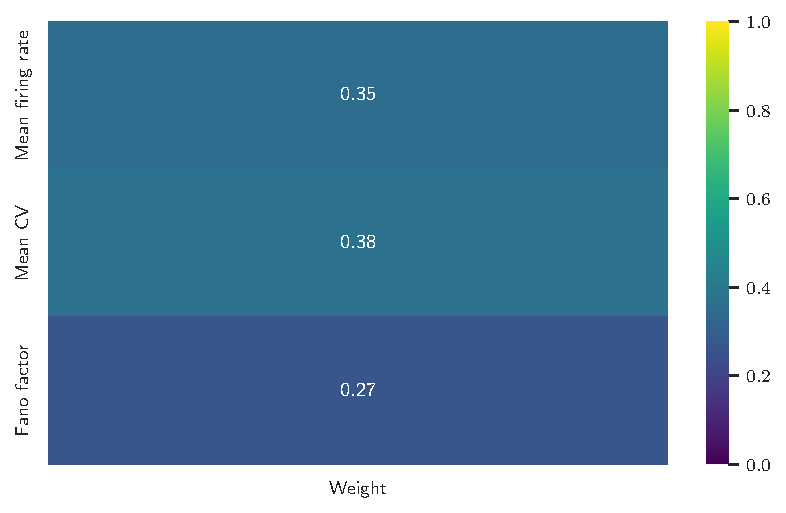
\includegraphics[scale=0.7]{brunel_sum_stats_weights}}}
\caption{\textbf{(a)} sum stats correlation. \textbf{(b)} sum stats weights
}
\label{fig:fig1}
\end{figure}

corr coefs of these particular summary statistics indicate that the AI state is most sensitive to the relative strength of inhibitory synapses $g$. Thus, we expect the summary statistics to constrain the $g$ parameter better.


\section{Posteriors} 

Ran 2000 simulations of the model with different parameters drawn from the priors. RMSPE vs quantile: 

\begin{figure}[H]
    \centering
    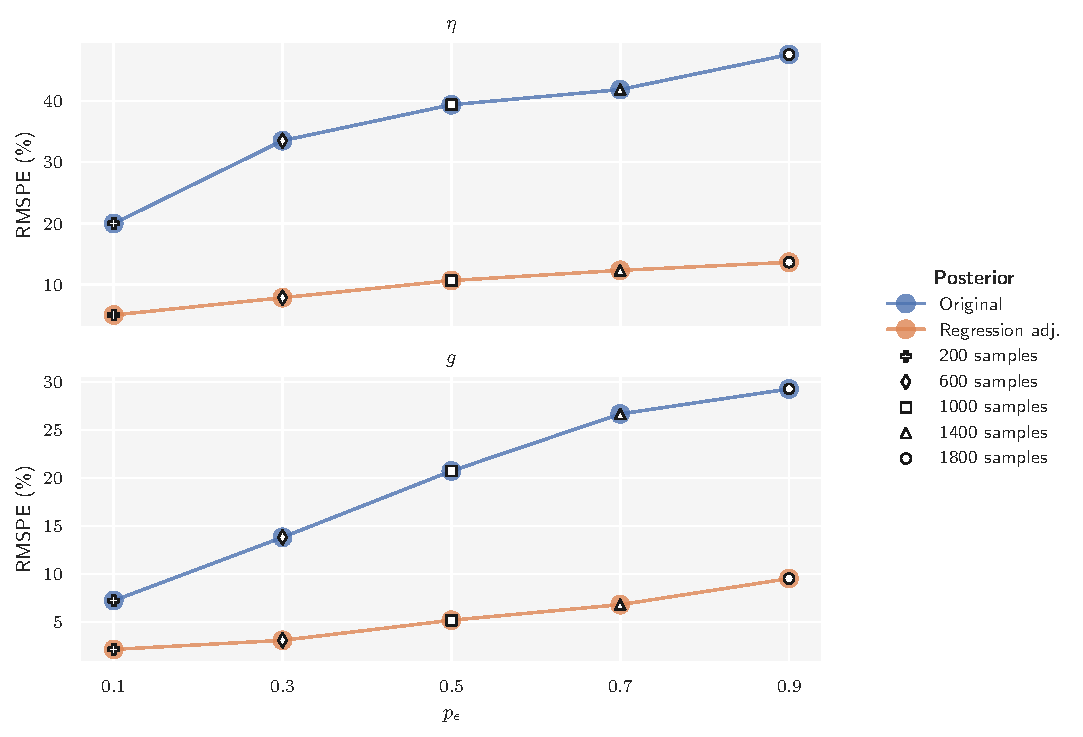
\includegraphics[scale=0.8]{brunel_quantile_rmspe}
    \caption{caption}
    \label{fig:fig1}
\end{figure}

Use 0.3-quantile, compromise between accuracy and number of samples in the posterior

original posterior

\begin{figure}[H]
    \centering
    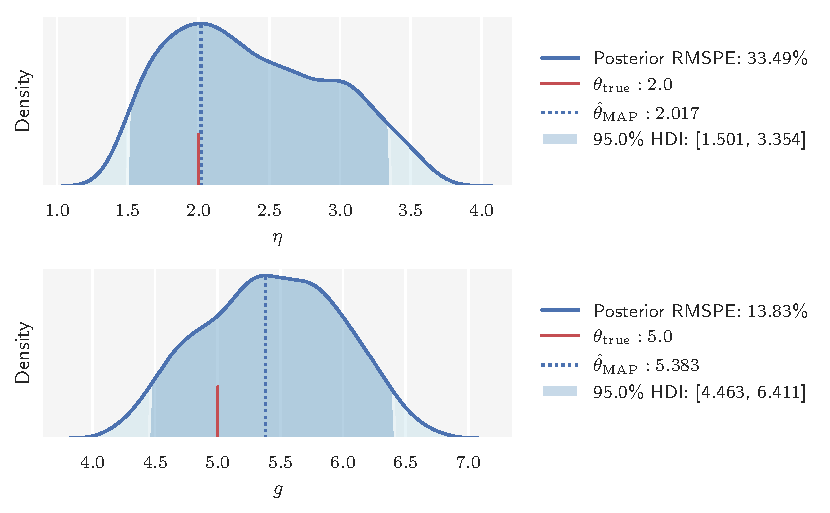
\includegraphics[scale=1.0]{brunel_posterior_org}
    \caption{caption}
    \label{fig:fig1}
\end{figure}

reg adjusted posterior

\begin{figure}[H]
    \centering
    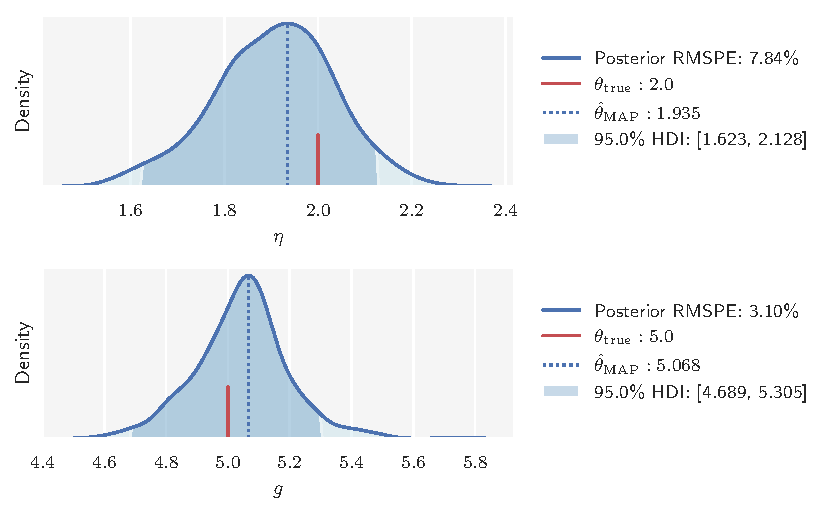
\includegraphics[scale=1.0]{brunel_posterior_reg}
    \caption{caption}
    \label{fig:fig1}
\end{figure}


joint posterior (reg adjusted)

\begin{figure}[H]
    \centering
    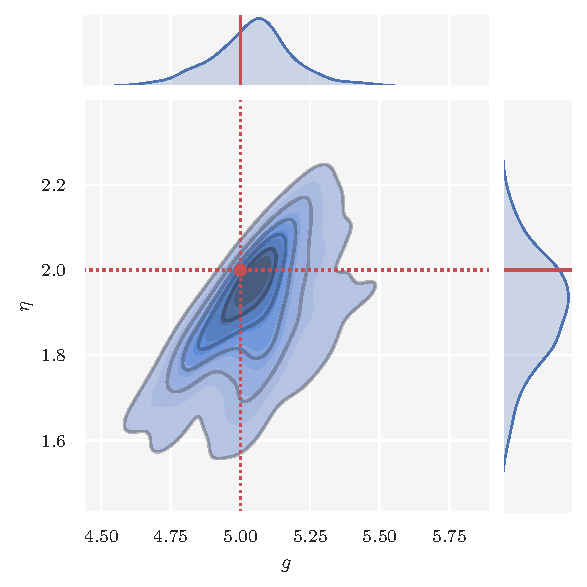
\includegraphics[scale=1.0]{brunel_joint_posterior_reg}
    \caption{caption}
    \label{fig:fig1}
\end{figure}

posterior predictive checks with reg adjusted samples, 50 samples from posterior pred

\begin{figure}[H]
    \centering
    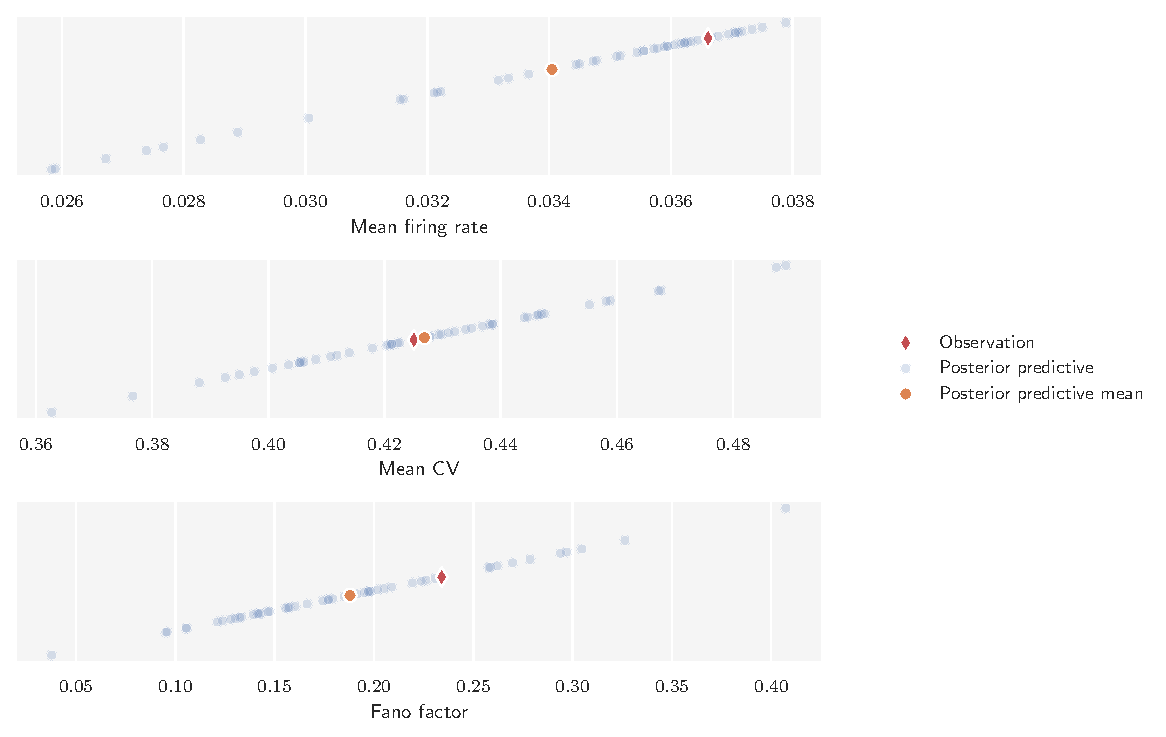
\includegraphics[scale=0.8]{brunel_post_pred}
    \caption{caption}
    \label{fig:fig1}
\end{figure}

The pairwise Pearson's correlation coefficient is a measure of how synchronous the spiking of a network is. This correlation coefficient measures the correlation between the spike trains of two neurons in the network. In Figure X we examine how this correlation depends on parameter uncertainties by plotting the mean and standard deviation for the pairwise Pearson's correlation coefficient in the AI state.

% subfigure
\begin{figure}[H]
\centering
\subfloat[]{{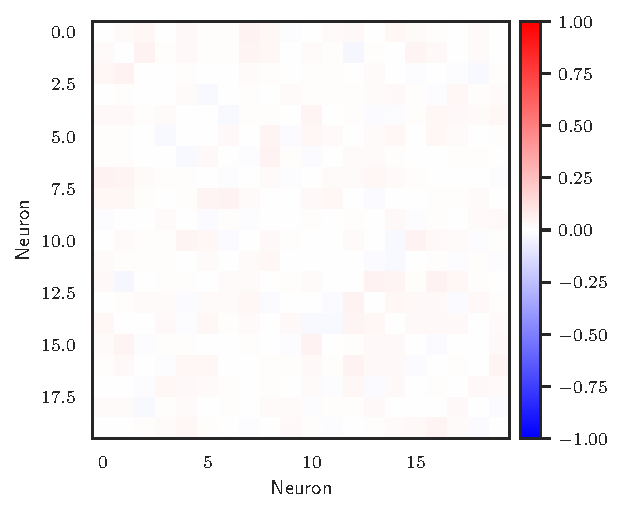
\includegraphics[scale=0.6]{brunel_pred_corr}}}
\qquad
\subfloat[]{{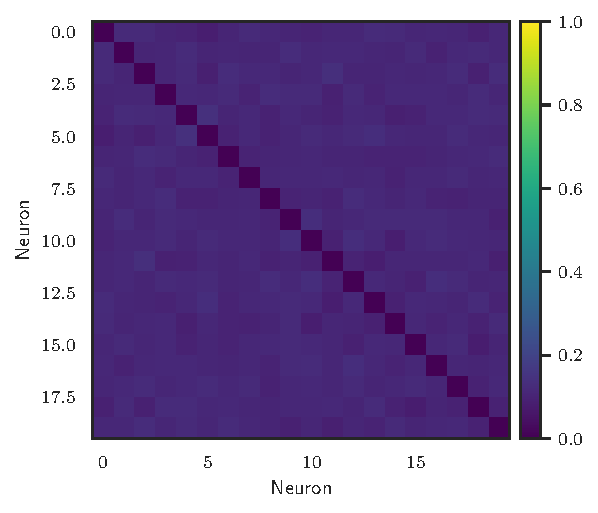
\includegraphics[scale=0.6]{brunel_pred_corr_std}}}
\caption{\textbf{(a)} mean correlation coefficient matrix. \textbf{(b)} standard deviation
}
\label{fig:fig1}
\end{figure}





%================================================================
\section{Brunel SBI Results}
%================================================================

%================================================================
\subsection{AI state} 
%================================================================



0.037222	0.401465	0.145315

Posterior:

\begin{figure}[H]
    \centering
    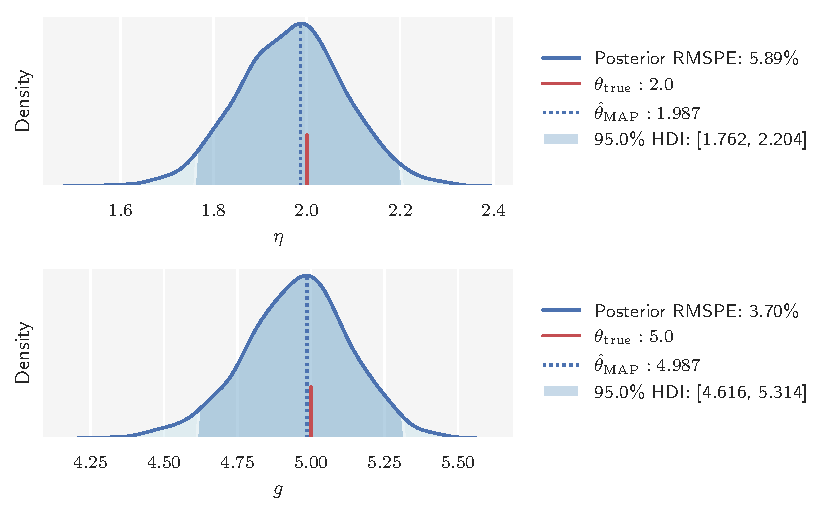
\includegraphics[scale=0.8]{brunel_post_ai_sbi}
    \caption{caption}
    \label{fig:fig1}
\end{figure}

ppc 

\begin{figure}[H]
    \centering
    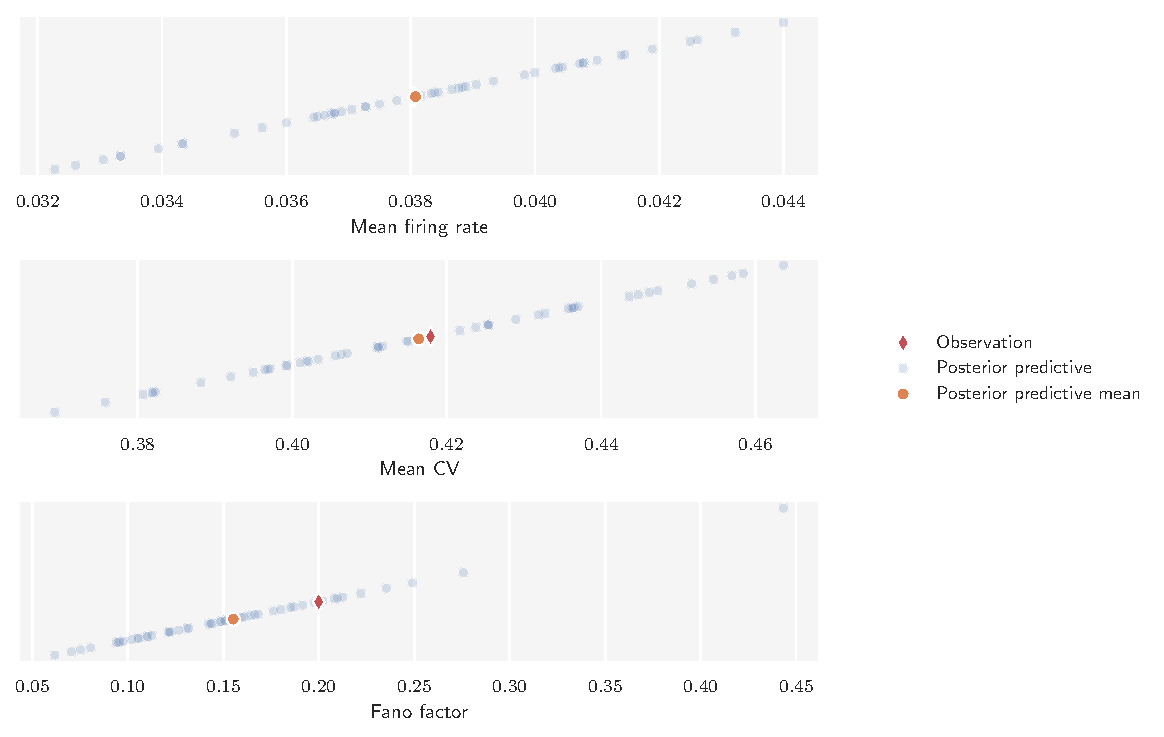
\includegraphics[scale=0.8]{brunel_post_pred_ai_sbi}
    \caption{caption}
    \label{fig:fig1}
\end{figure}

corr 

\begin{figure}[H]
    \centering
    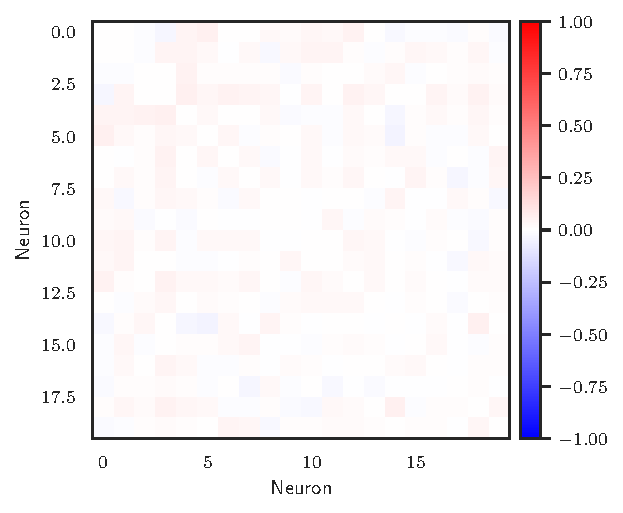
\includegraphics[scale=0.8]{brunel_pred_corr_sbi_ai}
    \caption{caption}
    \label{fig:fig1}
\end{figure}

corr std

\begin{figure}[H]
    \centering
    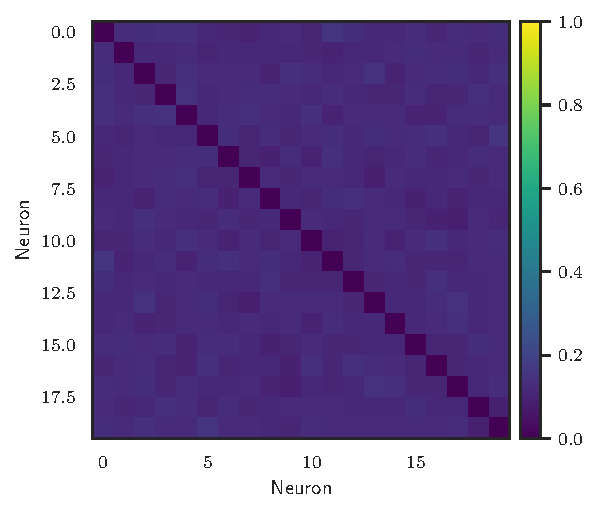
\includegraphics[scale=0.8]{brunel_pred_corr_std_ai_sbi}
    \caption{caption}
    \label{fig:fig1}
\end{figure}

%================================================================
\subsection{SR state}
%================================================================

SR observation

\begin{figure}[H]
    \centering
    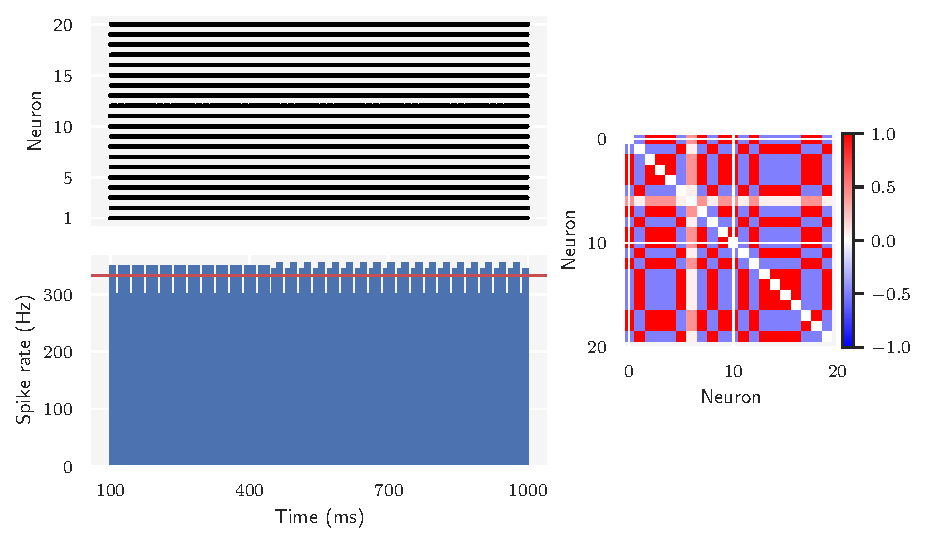
\includegraphics[scale=1.0]{brunel_sr_observation}
    \caption{caption}
    \label{fig:fig1}
\end{figure}

Recorded spike trains from the Brunel network and observed the following summary statistics:

\begin{table}[H]
  \caption{SR state observation.}
  %\footnotesize%
  \begin{center}
    \rowcolors{2}{gray!15}{white}
    \begin{tabular}{cc}
      \toprule
      \textbf{Summary statistic} & \textbf{Observed value} \\
      \midrule
      Mean firing rate &  0.3333 kHz \\
      Mean CV &  0.0121  \\
      Fano factor & 0.007  \\
      \bottomrule
    \end{tabular}
  \end{center}
  \label{tab:hh_noisy_sumstats}
\end{table}

Posterior:

\begin{figure}[H]
    \centering
    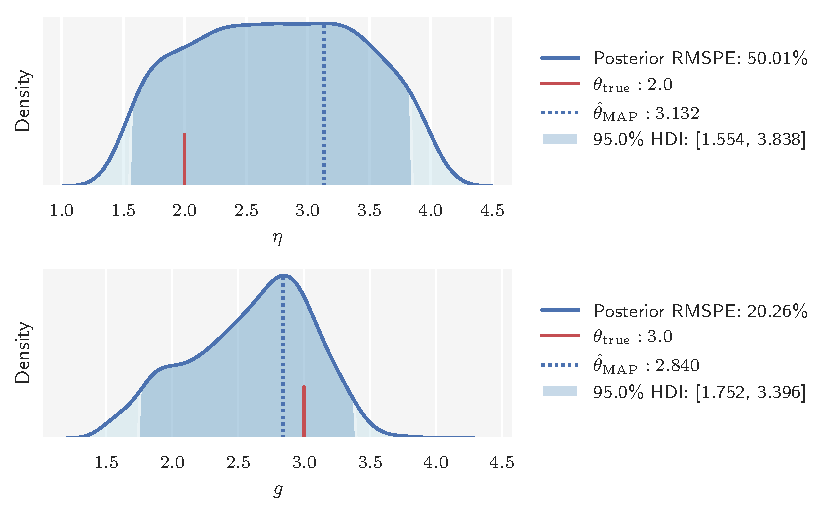
\includegraphics[scale=0.8]{brunel_post_sr_sbi}
    \caption{caption}
    \label{fig:fig1}
\end{figure}

ppc 

\begin{figure}[H]
    \centering
    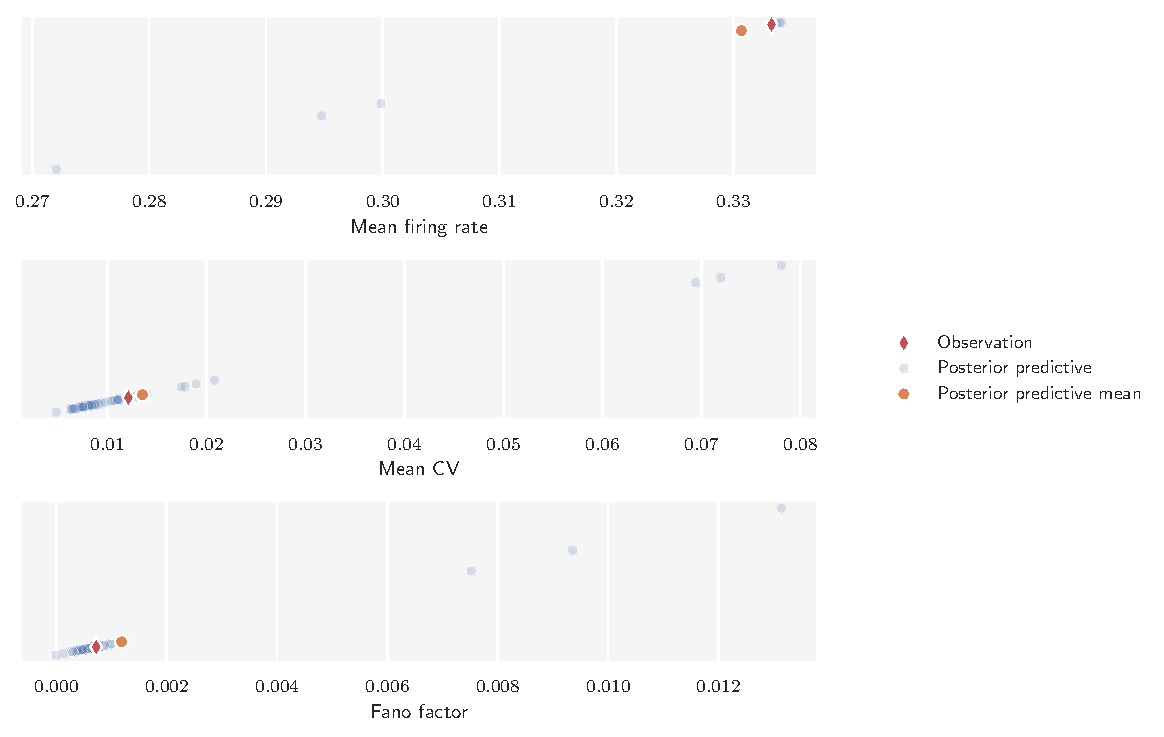
\includegraphics[scale=0.8]{brunel_post_pred_sr_sbi}
    \caption{caption}
    \label{fig:fig1}
\end{figure}

corr 

\begin{figure}[H]
    \centering
    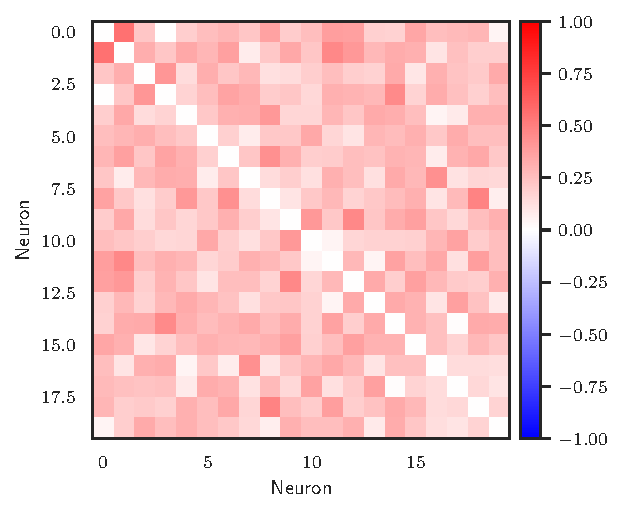
\includegraphics[scale=0.8]{brunel_pred_corr_sbi_sr}
    \caption{caption}
    \label{fig:fig1}
\end{figure}

corr std

\begin{figure}[H]
    \centering
    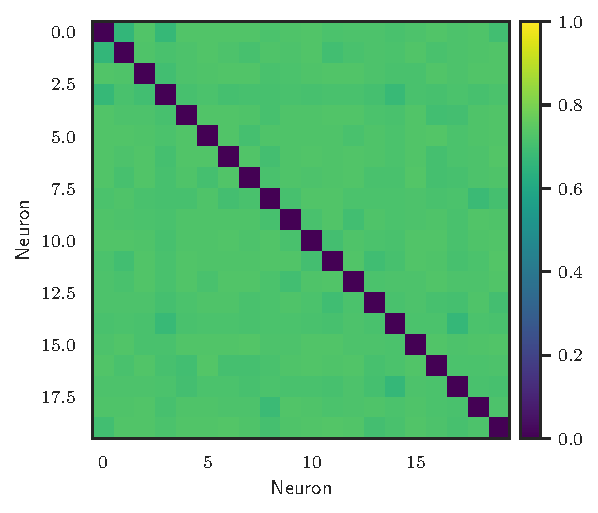
\includegraphics[scale=0.8]{brunel_pred_corr_std_sr_sbi}
    \caption{caption}
    \label{fig:fig1}
\end{figure}
